\documentclass[tikz,border=5pt]{standalone}
\usepackage{times}
\usepackage{amsmath,amssymb}
\usetikzlibrary{positioning,fit,arrows.meta,backgrounds,shapes.geometric,calc,shadows,decorations.pathreplacing}

\begin{document}
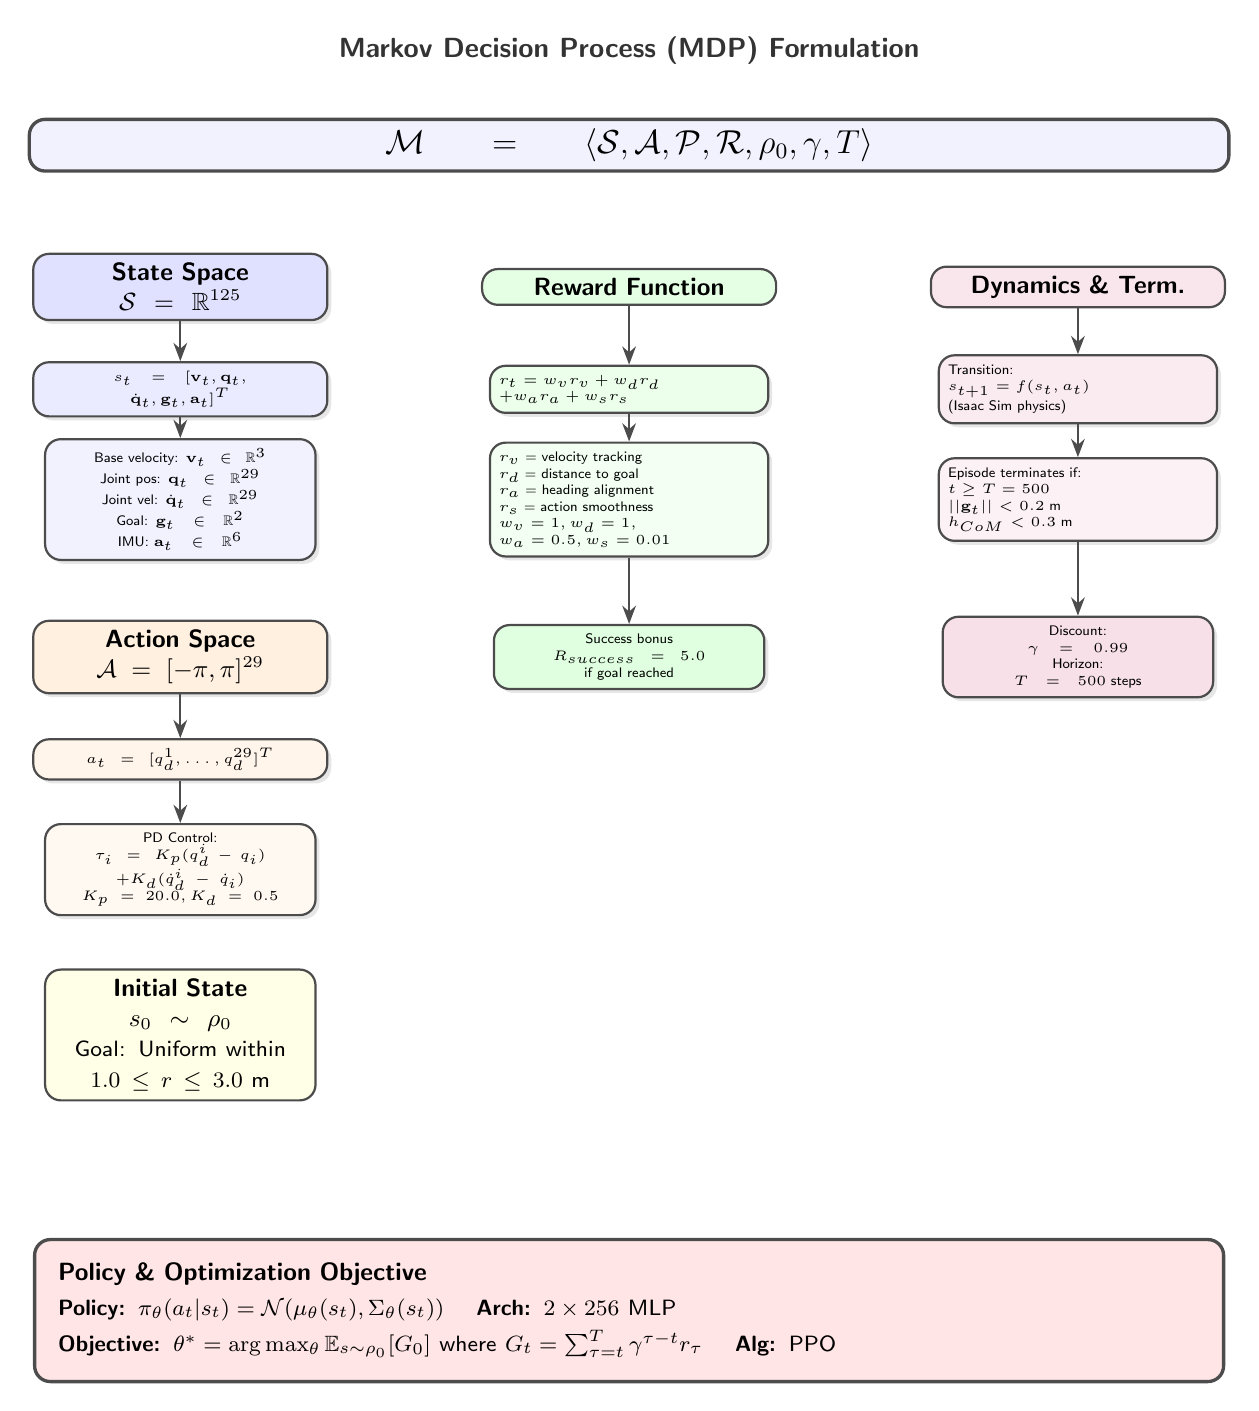
\begin{tikzpicture}[
    node distance=1.0cm and 1.5cm,
    box/.style={
        draw=black!70,
        rounded corners=2mm,
        fill=white,
        thick,
        font=\sffamily\small,
        align=center,
        drop shadow={opacity=0.2, shadow xshift=0.05cm, shadow yshift=-0.05cm}
    },
    header/.style={
        font=\sffamily\bfseries\normalsize,
        color=black!80
    },
    formula/.style={
        font=\ttfamily\footnotesize,
        color=black!70
    },
    arrow/.style={->, >=Stealth, thick, color=black!70},
    label/.style={font=\sffamily\tiny, color=black!60}
]

% ============================================================
% TITLE
% ============================================================
\node[header] at (7.5, 13.5) {Markov Decision Process (MDP) Formulation};

% ============================================================
% MDP TUPLE (TOP)
% ============================================================
\node[draw=black!70, rounded corners=2mm, fill=blue!5, very thick, text width=15cm, align=center] (mdp_tuple) at (7.5, 12.3) {
\large $\mathcal{M} = \langle \mathcal{S}, \mathcal{A}, \mathcal{P}, \mathcal{R}, \rho_0, \gamma, T \rangle$
};

% ============================================================
% STATE SPACE (LEFT)
% ============================================================
\node[box, fill=blue!12, text width=3.5cm] (state_header) at (1.8, 10.5) {\textbf{State Space}\\$\mathcal{S} = \mathbb{R}^{125}$};

\node[box, fill=blue!8, text width=3.5cm, font=\sffamily\tiny] (state_def) at (1.8, 9.2) {
$s_t = [\mathbf{v}_t, \mathbf{q}_t,$\\
$\dot{\mathbf{q}}_t, \mathbf{g}_t, \mathbf{a}_t]^T$
};

\node[box, fill=blue!5, text width=3.2cm, font=\sffamily\tiny] (state_comp) at (1.8, 7.8) {
Base velocity: $\mathbf{v}_t \in \mathbb{R}^3$\\
Joint pos: $\mathbf{q}_t \in \mathbb{R}^{29}$\\
Joint vel: $\dot{\mathbf{q}}_t \in \mathbb{R}^{29}$\\
Goal: $\mathbf{g}_t \in \mathbb{R}^2$\\
IMU: $\mathbf{a}_t \in \mathbb{R}^6$
};

% ============================================================
% ACTION SPACE (CENTER-LEFT)
% ============================================================
\node[box, fill=orange!12, text width=3.5cm] (action_header) at (1.8, 5.8) {\textbf{Action Space}\\$\mathcal{A} = [-\pi, \pi]^{29}$};

\node[box, fill=orange!8, text width=3.5cm, font=\sffamily\tiny] (action_def) at (1.8, 4.5) {
$a_t = [q_d^1, \ldots, q_d^{29}]^T$
};

\node[box, fill=orange!5, text width=3.2cm, font=\sffamily\tiny] (action_ctrl) at (1.8, 3.1) {
PD Control:\\
$\tau_i = K_p(q_d^i - q_i)$\\
$+ K_d(\dot{q}_d^i - \dot{q}_i)$\\
$K_p = 20.0, K_d = 0.5$
};

% ============================================================
% REWARD FUNCTION (CENTER)
% ============================================================
\node[draw=black!70, rounded corners=2mm, fill=green!10, thick, text width=3.5cm, align=center, font=\sffamily\small] (reward_header) at (7.5, 10.5) {\textbf{Reward Function}};

\node[box, fill=green!8, text width=3.3cm, font=\sffamily\tiny, align=left] (reward_eq) at (7.5, 9.2) {
$r_t = w_v r_v + w_d r_d$\\
$+ w_a r_a + w_s r_s$
};

\node[box, fill=green!5, text width=3.3cm, font=\sffamily\tiny, align=left] (reward_comp) at (7.5, 7.8) {
$r_v$ = velocity tracking\\
$r_d$ = distance to goal\\
$r_a$ = heading alignment\\
$r_s$ = action smoothness\\
$w_v=1, w_d=1,$\\
$w_a=0.5, w_s=0.01$
};

\node[box, fill=green!12, text width=3.2cm, font=\sffamily\tiny] (reward_bonus) at (7.5, 5.8) {Success bonus\\$R_{success} = 5.0$\\if goal reached
};

% ============================================================
% TRANSITION & TERMINATION (CENTER-RIGHT)
% ============================================================
\node[draw=black!70, rounded corners=2mm, fill=purple!10, thick, text width=3.5cm, align=center, font=\sffamily\small] (dyn_header) at (13.2, 10.5) {\textbf{Dynamics \& Term.}};

\node[box, fill=purple!8, text width=3.3cm, font=\sffamily\tiny, align=left] (dynamics) at (13.2, 9.2) {
Transition:\\
$s_{t+1} = f(s_t, a_t)$\\
(Isaac Sim physics)
};

\node[box, fill=purple!5, text width=3.3cm, font=\sffamily\tiny, align=left] (termination) at (13.2, 7.8) {
Episode terminates if:\\
$t \geq T = 500$\\
$||\mathbf{g}_t|| < 0.2$ m\\
$h_{CoM} < 0.3$ m
};

\node[box, fill=purple!12, text width=3.2cm, font=\sffamily\tiny] (discount) at (13.2, 5.8) {
Discount:\\
$\gamma = 0.99$\\
Horizon:\\
$T = 500$ steps
};

% ============================================================
% CONNECTIONS
% ============================================================
\draw[arrow] (state_header) -- (state_def);
\draw[arrow] (state_def) -- (state_comp);

\draw[arrow] (action_header) -- (action_def);
\draw[arrow] (action_def) -- (action_ctrl);

\draw[arrow] (reward_header) -- (reward_eq);
\draw[arrow] (reward_eq) -- (reward_comp);
\draw[arrow] (reward_comp) -- (reward_bonus);

\draw[arrow] (dyn_header) -- (dynamics);
\draw[arrow] (dynamics) -- (termination);
\draw[arrow] (termination) -- (discount);

% ============================================================
% POLICY & OPTIMIZATION (BOTTOM)
% ============================================================
\node[draw=black!70, rounded corners=2mm, fill=red!10, very thick, text width=14.5cm, minimum height=1.8cm, align=left, font=\sffamily\small, inner sep=0.3cm] (policy_box) at (7.5, -2.5) {
\textbf{Policy \& Optimization Objective}\\[3pt]
\footnotesize
\textbf{Policy:} $\pi_\theta(a_t | s_t) = \mathcal{N}(\mu_\theta(s_t), \Sigma_\theta(s_t))$ \quad \textbf{Arch:} $2 \times 256$ MLP\\[2pt]
\textbf{Objective:} $\theta^* = \arg\max_\theta \mathbb{E}_{s \sim \rho_0} [G_0]$ where $G_t = \sum_{\tau=t}^{T} \gamma^{\tau-t} r_\tau$ \quad \textbf{Alg:} PPO
};

% ============================================================
% INITIAL STATE DISTRIBUTION (BOTTOM-LEFT)
% ============================================================
\node[draw=black!70, rounded corners=2mm, fill=yellow!10, thick, text width=3.2cm, align=center, font=\sffamily\small] (init_box) at (1.8, 1.0) {
\textbf{Initial State}\\
$s_0 \sim \rho_0$\\
\vspace{3pt}
\fontsize{8}{8}\selectfont
Goal: Uniform within\\
$1.0 \leq r \leq 3.0$ m
};

\end{tikzpicture}
\end{document}
